\documentclass[10pt,executivepaper]{article}
\usepackage[utf8]{inputenc}
\usepackage[spanish]{babel}
\usepackage{amsmath}
\usepackage{amsfonts}
\usepackage{amssymb}
\usepackage{graphics}
\usepackage{graphicx}
\usepackage[left=2cm,right=2cm,top=2cm,bottom=2cm]{geometry}
\usepackage{imakeidx}
\makeindex[columns=3, title=Alphabetical Index, intoc]
\usepackage{listings}
\usepackage{xcolor}
\usepackage{multicol}
\usepackage{changepage}
\usepackage{float}
\usepackage{cite}
\usepackage{url}
\usepackage{pdflscape}

\definecolor{codegreen}{rgb}{0,0.6,0}
\definecolor{codegray}{rgb}{0.5,0.5,0.5}
\definecolor{codepurple}{rgb}{0.58,0,0.82}
\definecolor{backcolour}{rgb}{0.95,0.95,0.92}

\lstdefinestyle{mystyle}{
    backgroundcolor=\color{backcolour},
    commentstyle=\color{codegreen},
    keywordstyle=\color{magenta},
    numberstyle=\tiny\color{codegray},
    stringstyle=\color{codepurple},
    basicstyle=\ttfamily\footnotesize,
    breakatwhitespace=false,
    breaklines=true,
    captionpos=b,
    keepspaces=true,
    numbers=left,
    numbersep=5pt,
    showspaces=false,
    showstringspaces=false,
    showtabs=false,
    tabsize=3
}
\def\fillandplacepagenumber{%
 \par\pagestyle{empty}%
 \vbox to 0pt{\vss}\vfill
 \vbox to 0pt{\baselineskip0pt
   \hbox to\linewidth{\hss}%
   \baselineskip\footskip
   \hbox to\linewidth{%
     \hfil\thepage\hfil}\vss}}
\lstset{style=mystyle}

\title{Actividad: Matrices Distribuidas}

\author{Instituto Politécnico Nacional\\Escuela Superior de Computo\\Desarrollo de Sistemas Distribuidos\\Adrian González Pardo\\4CV1\\21/01}
\date{23 de octubre de 2020}
\newcommand\tab[1][1cm]{\hspace*{#1}}

\begin{document}
\maketitle
\section{Código fuente:}
\begin{center}
  \lstinputlisting[language=Java]{../Matriz.java}
  \lstinputlisting[language=Bash]{../Makefile}
\end{center}
\section{Capturas y descripción del programa}
\begin{center}
  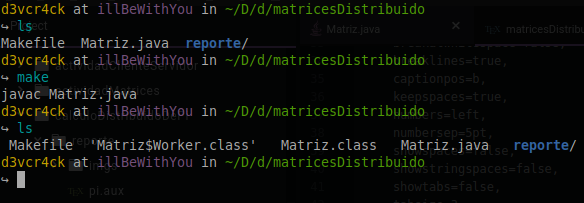
\includegraphics[scale=0.5]{imgs/compilacion.png}
  \\\textit{En esta captura podemos ver la compilación rapida del archivo Matriz.java gracias al archivo y las tareas que realiza el archivo Makefile y la sencillez de simplemente escribir make en la terminal}

  \begin{landscape}
    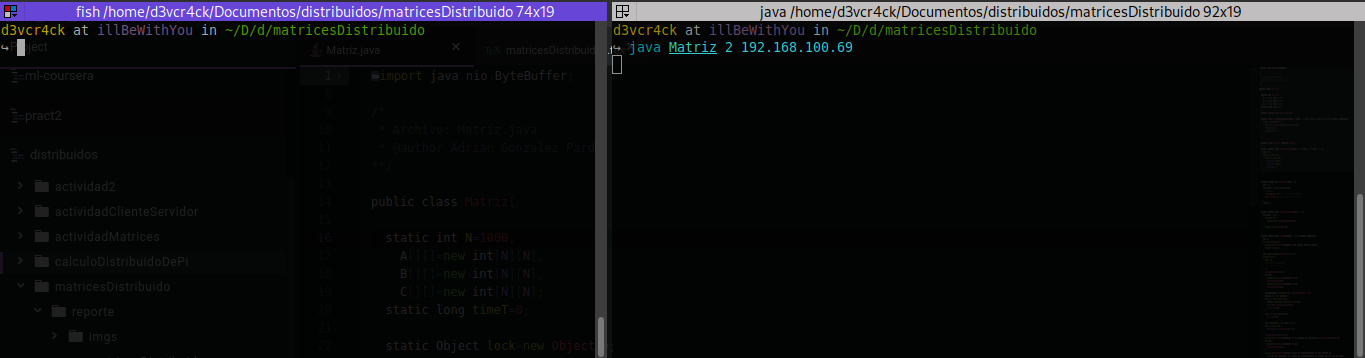
\includegraphics[scale=0.5]{imgs/terminal-sin-server.png}
    \\\textit{En esta captura vemos que los nodos clientes se pueden ejecutar aun sin la existencia del servidor}
    \fillandplacepagenumber
    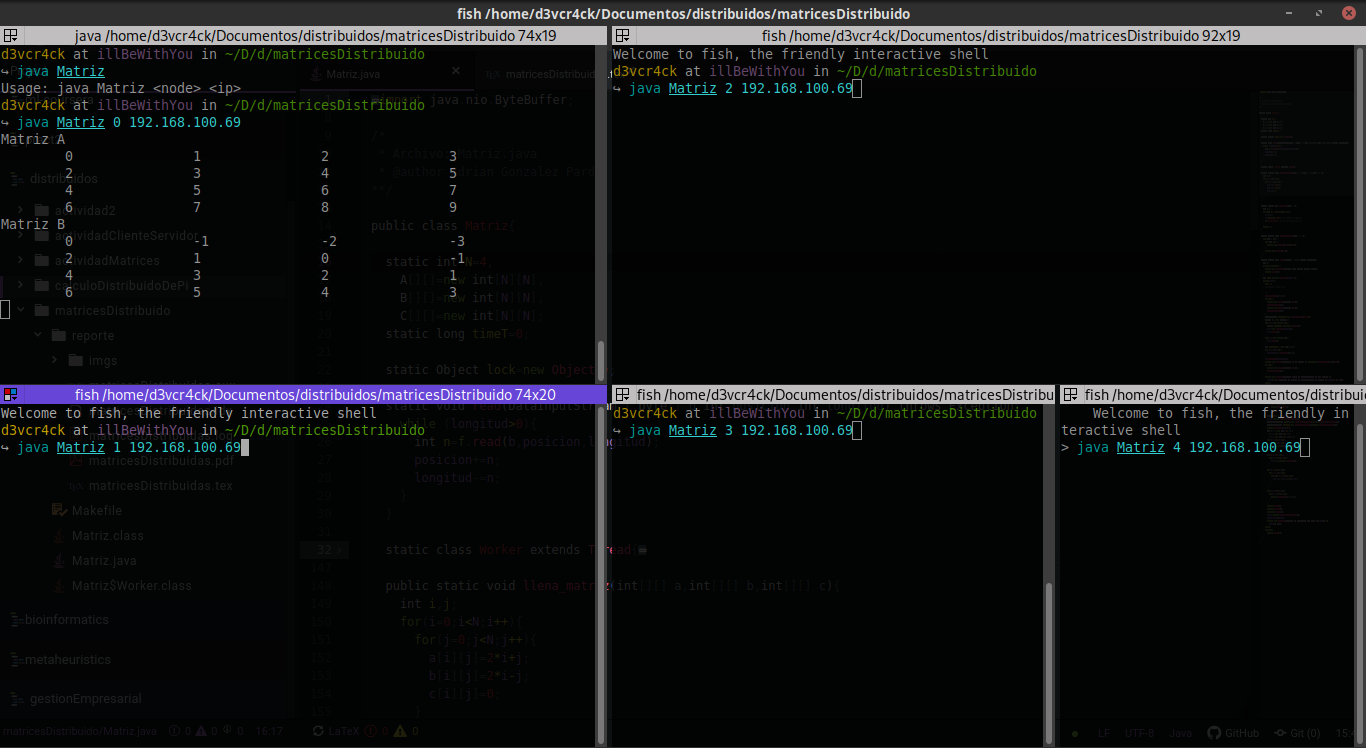
\includegraphics[scale=0.45]{imgs/terminal-1.png}
    \\\textit{En esta captura vemos que el server queda en espera de los clientes}
    \fillandplacepagenumber

  \end{landscape}

  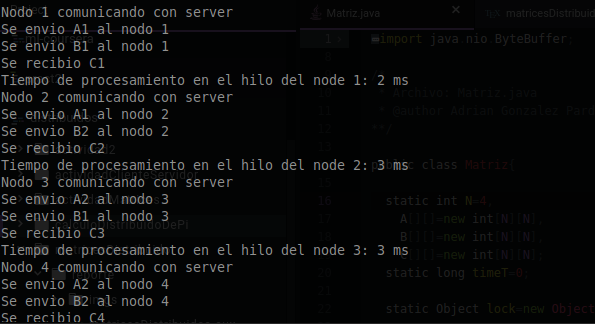
\includegraphics[scale=0.5]{imgs/ejec-nodo0.png}
  \\\textit{En esta captura vemos la ejecución del servidor una vez que los clientes recibieron y enviaron sus datos con una matriz de 4x4.}

  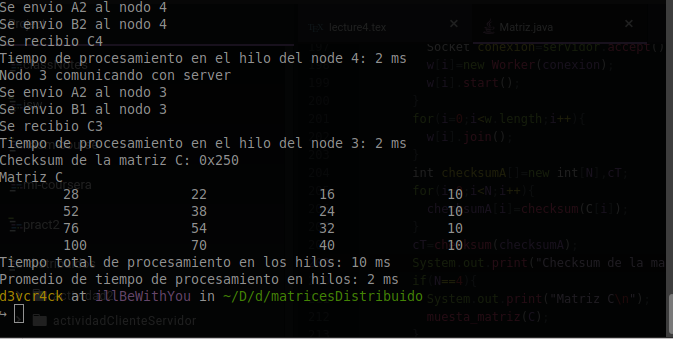
\includegraphics[scale=0.5]{imgs/checksum.png}
  \\\textit{En esta captura vemos la continuación de la captura anterior.}

  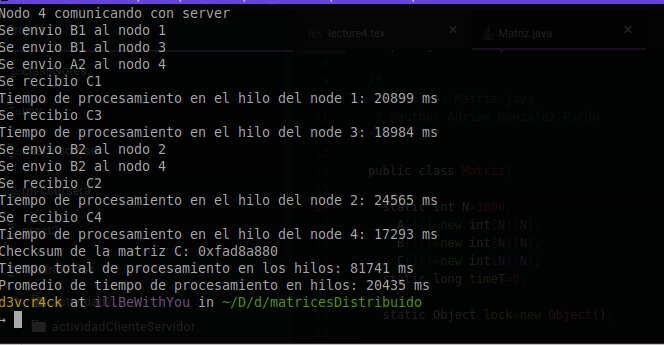
\includegraphics[scale=0.5]{imgs/checksum-1.png}
  \\\textit{En esta captura vemos la ejecución del programa con una matriz de 1000x1000 datos.}

\end{center}
\end{document}
